% Member 4 - Section 3.7 Experimental Design and Fair Comparison
\subsection{Experimental Design and Fair Comparison}
\label{sec:exp_design}

\textit{Experiments.} Five experiments answer the research questions in the Introduction. Experiment 1 trains the Original group and measures the Photo-versus-target gap. Experiment 2 compares Original against +AdaIN. Experiment 3 compares +AdaIN against +Ours with everything else held fixed. Experiment 4 sweeps the style strength $\alpha \in \{0.25, 0.5, 0.75, 1.0\}$ for both augmentation methods, tracing the relation between stylization strength, structure preservation, and cross-domain accuracy. A $\beta$ ablation for the structure-preserving method is planned alongside Experiment 4 (Section~5.3). Experiment 5 is the control that makes Experiment 3 interpretable: it isolates the effect of the \emph{spatial} modulation from the effect of the \emph{overall style strength}, which the two differ in simultaneously.

\textit{Why a strength control is necessary.} The structure-preserving map is $\alpha(x,y) = \alpha_0(1-\beta M)$, so wherever $M$ is large the applied strength is necessarily below $\alpha_0$. The spatial map therefore always carries \emph{less} total style than a uniform AdaIN at the same $\alpha_0$: at our main setting ($\alpha_0 = 0.5$, $\beta = 0.7$) its mean is $0.374$, against $0.500$ for the uniform mix. A direct comparison of +AdaIN against +Ours consequently changes two things at once---the spatial modulation and the overall style strength---and a difference in accuracy cannot be attributed to either alone. We resolve this with two additional controls, both trained under the identical protocol:

\begin{itemize}
\item \textit{Strength-matched uniform AdaIN.} A plain uniform AdaIN whose strength is, for each image individually, the mean of that image's spatial $\alpha$ map. It has the same total style energy as the spatial map and differs from it only in that the strength is not modulated in space.
\item \textit{Equal-strength spatial map.} The $\alpha_0$ is recalibrated so that the spatial map's mean is exactly $0.500$, matching the uniform AdaIN at $\alpha = 0.5$ to four decimals: with $\beta = 0.7$ and $\overline{M} = 0.361$, this requires $\alpha_0 = 0.500 / (1 - 0.7 \times 0.361) = 0.6692$. Here +Ours and +AdaIN differ in the spatial modulation and in nothing else.
\end{itemize}

Both controls use the same style pool, the same frozen content--style pairing, the same seeds, the same step budget, and the same classifier, and both are verified by the fairness checker before training.

\textit{Fairness controls.} Because the compared methods differ only in their training images, the following quantities are fixed across groups:

\begin{itemize}
\item \textit{Same original data:} all groups train on the identical 1{,}349 Photo Training images from Table~\ref{tab:splits}.
\item \textit{Same style pool:} both augmented groups draw style references from one frozen pool of 10 style images, fixed with a content-hash manifest before any training run. The pool holds external paintings that are not part of PACS, and the checker verifies this mechanically (the ``No test-set leakage'' item below).
\item \textit{Same augmentation count:} each augmented group adds exactly one stylized image per original training image (1{,}349 added images).
\item \textit{Same content--style pairing:} the style image paired with each content image is drawn once with a fixed seed and reused by both generators, so the only difference between the two augmented datasets is the stylization algorithm itself.
\item \textit{Same transform pipeline and classifier:} one training script, one transform definition, one ResNet-18 configuration for all groups.
\item \textit{Same optimization budget:} all groups receive the same number of optimizer steps, $S = 660$, computed as 30 passes over the Original training set at batch size 64 ($30 \times 22$). Groups with larger training sets accordingly run fewer passes over their data. Validation is evaluated at the same step cadence for every group.
\item \textit{Same evaluation and seeds:} all groups use the test lists of Table~\ref{tab:splits} and are run with seeds $\{0, 1, 2\}$.
\item \textit{No checkpoint selection:} the reported model is the final checkpoint of the fixed step budget, for every group and every seed. This removes a selection step that we measured to be harmful (Section~\ref{sec:resnet_baseline}).
\item \textit{No test-set leakage:} the style pool is built from external paintings and contains no PACS image. Because Art Painting, Cartoon, and Sketch are the evaluation domains, a style reference drawn from any of them would place the test appearance into the training set. The checker compares the content hash of every style image against the whole local PACS copy and rejects the run if any style image is a PACS image.
\item \textit{Fairness verification.} A checker script validates these constraints mechanically before training: it confirms that the augmented manifests contain the same original images, the same style pool hash, the same augmentation count, that the content--style pairing is identical in both manifests, that no style image is a PACS image, and that the training configuration fingerprint is identical across groups. The configuration fingerprint is recomputed from the full training configuration recorded in each run summary, so a run whose hyper-parameters differ is rejected. A run that fails any check is excluded from results.
\end{itemize}

\textit{Reporting.} Table~\ref{tab:results} shows the result table format used throughout. Entries are mean$\pm$standard deviation over three seeds. Differences between groups are reported per seed, so that a gain which depends on one favorable seed is visible rather than hidden in the average. Because all groups share the same seeds, the design is \emph{paired}, and we report paired $t$ tests with 95\% confidence intervals rather than independent-samples tests; at three seeds this is the more powerful choice, and it is the only honest one at this sample size.

\begin{table}[t]
\caption{Result table. Entries are mean$\pm$standard deviation over three training seeds (final checkpoint of the fixed 660-step budget). The last two rows are the controls that separate the effect of the spatial modulation from the effect of the overall style strength.}
\label{tab:results}
\centering
\scriptsize
\setlength{\tabcolsep}{2.0pt}
\begin{tabular}{@{}lccccc@{}}
\toprule
Training method & Photo & Art & Cartoon & Sketch & Avg \\
\midrule
Original & $99.0\pm0.3$ & $63.2\pm3.7$ & $25.1\pm1.8$ & $31.5\pm4.2$ & $39.9\pm2.7$ \\
+AdaIN   & $99.2\pm0.3$ & $69.0\pm0.7$ & $32.2\pm1.7$ & $40.2\pm1.3$ & $\mathbf{47.1\pm0.8}$ \\
+AdaIN (matched) & $99.4\pm0.0$ & $68.0\pm1.3$ & $29.7\pm1.2$ & $38.4\pm2.5$ & $45.4\pm0.3$ \\
+Ours    & $99.8\pm0.3$ & $68.5\pm0.6$ & $30.0\pm0.9$ & $36.7\pm3.9$ & $45.1\pm1.5$ \\
+Ours (eq.\ strength) & $99.6\pm0.3$ & $68.1\pm0.8$ & $31.1\pm0.3$ & $41.8\pm3.3$ & $\mathbf{47.0\pm0.9}$ \\
\bottomrule
\end{tabular}
\end{table}

Experiment 1 is complete. The Original group reaches $99.0\%$ on Photo Test but only $39.9\%$ averaged over the three unseen domains, so the domain gap is both large and unambiguous. The gap is not uniform: Art Painting, whose appearance is closest to photography, is recognized at $63.2\%$, whereas Cartoon and Sketch, which discard most photographic cues, fall to $25.1\%$ and $31.5\%$. This ordering is the one we would expect from a classifier that relies mainly on photographic texture, and it identifies Cartoon and Sketch as the domains where style augmentation has the most room to help.

Experiment 2 shows that style augmentation itself is effective: adding 1{,}349 AdaIN-stylized images lifts the cross-domain average from $39.9\%$ to $47.1\%$, a gain of $7.2$ points, and it does so while \emph{reducing} the seed-to-seed spread from $2.7$ to $0.8$ points. The variance reduction matters as much as the mean: augmentation does not merely raise the expected accuracy, it makes the outcome reproducible, which is the property a single-seed result cannot show. The gain is consistent across all three target domains and is largest on Sketch ($+8.7$), the domain furthest from the source.

Experiments 3 and 5 give a clear and, we think, more interesting answer than a simple win would have. Against +AdaIN, +Ours does \emph{not} improve accuracy: the paired difference is $-2.0$ points ($t=-3.21$, $p=0.085$) at the main setting and $-0.3$ points ($p=0.81$) against the strength-matched control. The strength-matched control explains why: uniform AdaIN at the same mean strength scores $45.4\%$, i.e.\ $1.8$ points \emph{below} uniform AdaIN at full strength. The accuracy of these groups is governed almost entirely by how much style is applied, not by how that style is distributed in space. The equal-strength spatial map confirms this directly: with the mean strength pinned to $0.500$, it reaches $47.0\%$ against +AdaIN's $47.1\%$, a paired difference of $-0.1$ points ($p=0.89$)---the two methods are indistinguishable once strength is held fixed.

The mechanism itself does work, but not in the way the classification metric can see. Measured on all 1{,}349 images with paired per-image comparison, the spatial map retains more of the content's edge structure than plain AdaIN ($0.344$ against $0.321$, mean difference $+0.023$, 95\% CI $[+0.022, +0.023]$, $p<10^{-290}$), and its perceptual distance to the content is lower ($0.226$ against $0.279$). Against the strength-matched control, however, the difference \emph{reverses} slightly ($-0.003$, $p<10^{-22}$): the uniform mix at equal strength retains marginally more edges than the spatial map. The spatial modulation therefore does not deliver superior edge preservation once the confound is removed; what it does deliver is weaker stylization, and weaker stylization preserves edges for the trivial reason that less styling destroys fewer of them. Consistent with this, the per-image gain over the strength-matched control does not concentrate on structurally dense images (Spearman $\rho = +0.078$ against edge count; $-0.003$ in the dense half against $-0.003$ in the sparse half), so the mechanism the method is designed around is not observable in the images either.

\begin{figure}[t]
\centering
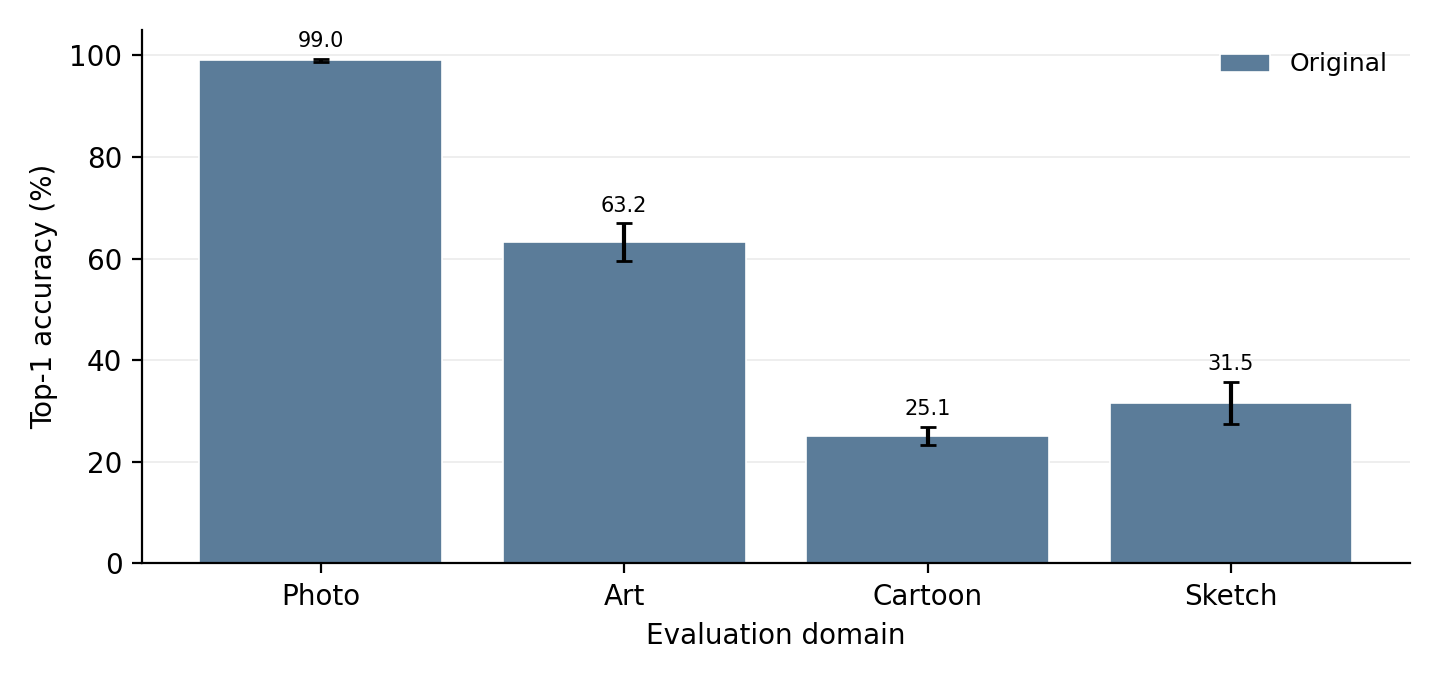
\includegraphics[width=\columnwidth]{figures/results_baseline.png}
\caption{Experiment 1: accuracy of the Original group on the in-domain Photo test set and on the three unseen target domains. Bars are means over three seeds; whiskers are standard deviations.}
\label{fig:results_baseline}
\end{figure}

%==================================================
